\section{Results}
\label{Results}
%\section{Data Analysis}
%\label{Data Analysis}

\subsection{Vertical Radiation Profile}
\begin{figure}[H]
\centering
\begin{subfigure}{.5\textwidth}
  \centering
  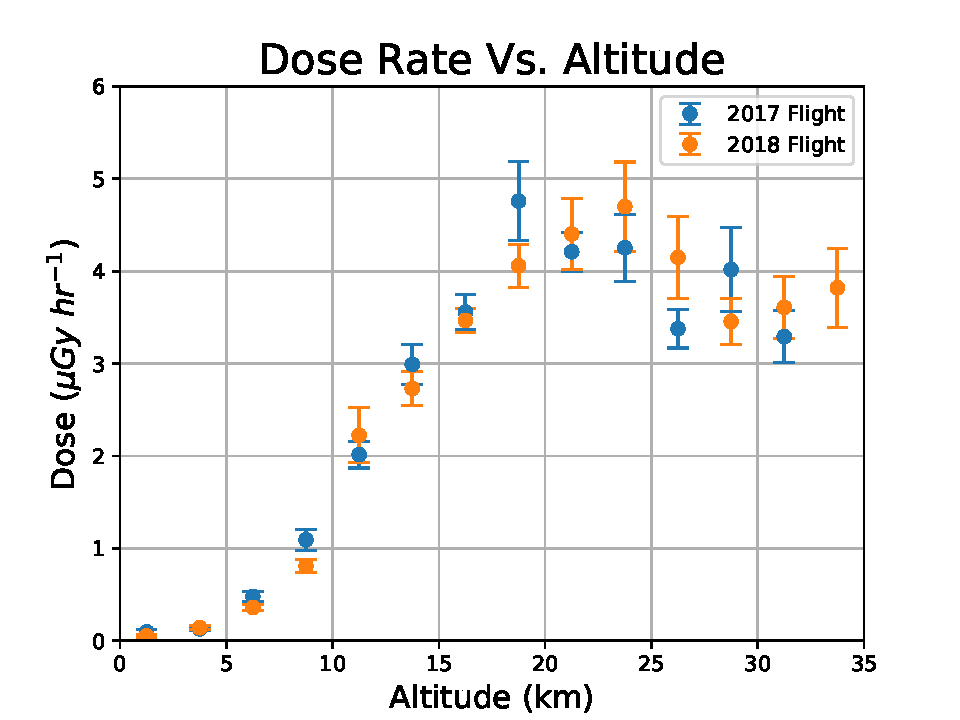
\includegraphics[scale=.45]{dva_stderr.pdf}
  \caption{Dose rate in silicon vs. altitude.}
  \label{fig:sub1}
\end{subfigure}%
\begin{subfigure}{.5\textwidth}
  \centering
  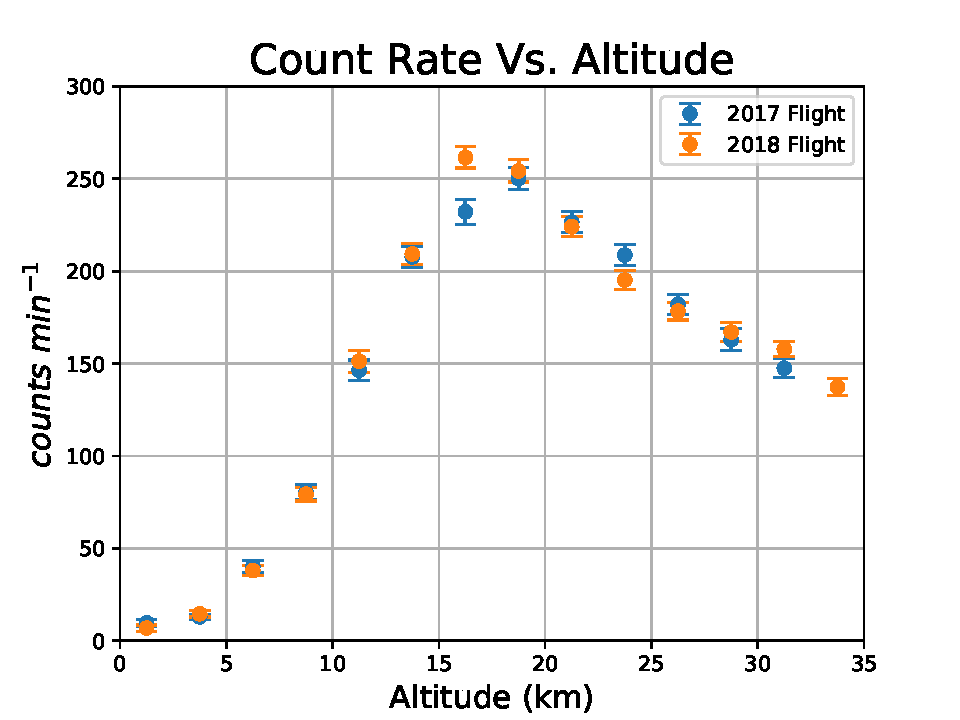
\includegraphics[scale=.45]{cva_stderr.pdf}
  \caption{Detector Hits vs. altitude.}
  \label{fig:sub2}
\end{subfigure}
\caption{Figure ~\ref{fig:sub1} shows the absorbed dose rate per hour as a function of altitude from the MiniPIX.  Figure ~\ref{fig:sub2} shows the counts per minute as a function of altitude again from the MiniPIX data.}
\label{fig:test}
\end{figure}

\begin{figure}[H]
\centering
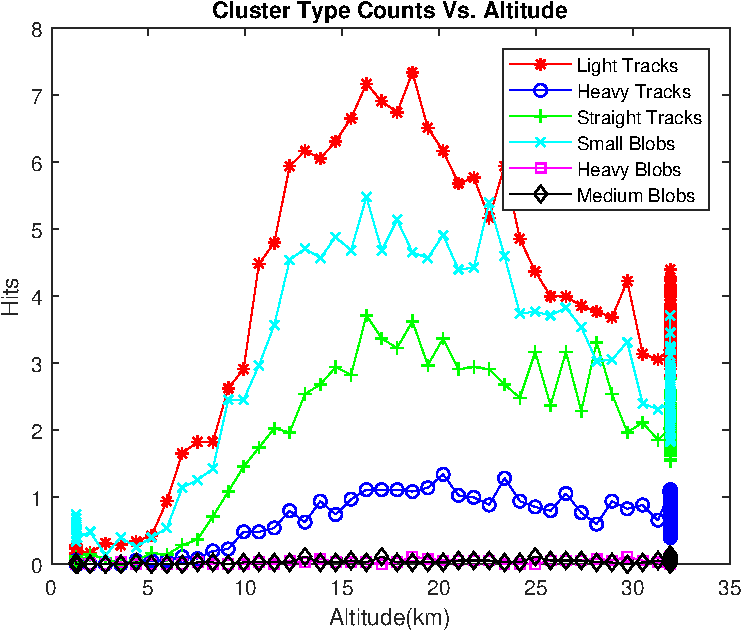
\includegraphics[scale=.5]{ctva-cropped.pdf}
\caption{Cluster Type Counts vs. altitude.}
\end{figure}

\begin{figure}[H]
\centering
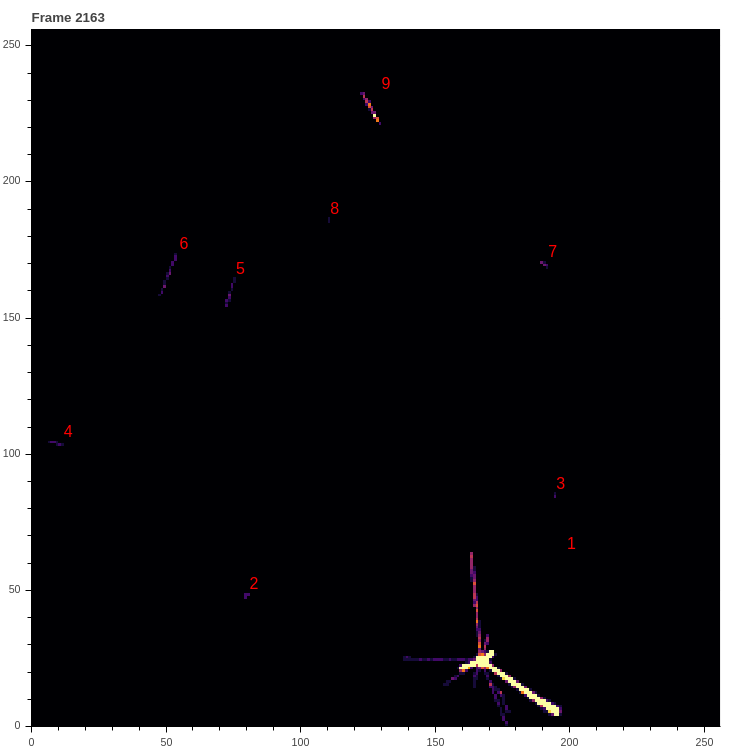
\includegraphics[scale=.35]{tracks.png}
\caption{Frame collected at float.}
\end{figure}
%Notes on how to take the results...
%What is being presented: Five plots total, the flight profile for each year, and cumulative dose for each flight.
%Present and characterize the first two plots - the data of the flight with counts vs altitude vs time.  Here we can talk about each flight and data shown.  Make sure to mention how the count rate changed as time and altitude changed.  We can talk about the flight time, the flight altitude variance, the coasting altitude, and how it all compares to the count rate.  We can be as descriptive as we can.
%mention the position of the pfotzer-regener maximum for both years.  Talk about discrepancies as the data shows.  Speculate in discussion later.
%Next, go into the absorbed rate vs altitude plot.  Mention how the LET varies for materials such as silicon and muscle.  Go into the pfotzer-regener maximum again, compare.  Compare this to the accompanying figure, Detector Hits vs Altitude.  There is a slight discrepancy in the flights, this may be useful to mention.  All error bars are 1 sigma standard deviation.
%Finally, the last figure Cluster Type Counts vs Altitude.  This is useful due to the MiniPIX being able to analyze indivudual track lenghts.  From here, these tracks can be characterized into different and indidivual categories.  This is useful for LET calculations and overall more precise for dosage calculations.  It may also help with particle identification.  Notice how the heavier tracks and medium blobs are all in the low counts yet they still vary somewhat with altitude (hard to see).
